% !TEX root = ../thesis-example.tex
%
\chapter{Implementation}
\label{sec:implementation}
%\vspace{-4em}{

The development of this web app can be split into three significant processes. The information and communications process which instated the backbone of controlling, gathering and communicating data. The bot process which is derived of three concurrent \textit{`actor'} models to gather and process Binance exchange data, then forwarding the generated signal results to the correct user. Finally, the front end process that can present information visually to an end user while allowing control over a bot's configurations and operations.

\section{Information \& Communication Process}
\label{sec:implementation:info_comm}

\noindent As stated in the aims of this project (Sec. \ref{sec:intro:aims}, pg. \pageref{sec:intro:aims}), the core services of the bot would be delivered as a web app using SaaS. The initial design choice of using a Flask web server was used to implement the communications backbone of the project. Extensions available to Flask allowed for extra functionality to be slotted into the web server. The extensions used in this project include Flask-RESTful that allowed the implementation of a REST API, Flask-SocketIO that allowed streaming two way communication between the server and client using WebSockets, and lastly Flask-SQLAlchemy that allowed a lightweight SQLite database to store meta data for server management purposes. These extensions are used to create endpoints to retrieve Binance exchange data from, as well as communicate with existing or create new instances of bots.

\subsection{Binance Exchange Data}
\label{sec:implementation:info_comm:binance_exchange_data}

% required to fulfil FR-3, FR-8, NFR-2

% TODO maybe use this in conclusion of impementation?
%\noindent The goal to developing the project's web server was to provide all endpoints for data requests in one place. This meant that, as well as allowing the developed front end UI to communicate with the web server, it is also open and available to all other software that can communicate with HTTP endpoints. 


% TODO include larger discussion of WebSockets as its a main technology in this application
\noindent During development, I initially discovered that modern browsers have security measures against directly requesting data that origins from external domains like \textit{http://api.binance.com}. This prevents a web vulnerability known as \textit{\textbf{Cross Site Scripting}} that while not specifically relevant to this project, was an obstacle in development. A solution to this problem is to proxy the data requests through the web server that would forward the data with the correct configurations; as to let the web browser accept the incoming data that origins from external domains. This restriction adheres to all request protocols except the WebSocket protocol, however to ensure consistency towards the origin point of accessing Binance's data, I also implemented WebSocket endpoints into the web server.

WebSockets and REST APIs were used to forward market data from the web server to the UI and the bot's data gatherer (See sec. \ref{sec:implementation:bot}, pg. \pageref{sec:implementation:bot}). The data endpoints that were required and offered by Binance were wrapped by Sam McHardy's \cite{MISC:Python-Binance} Python-Binance wrapper. This allowed for accessing this data through a function call that provided the required arguments to access a coin pair's data. The endpoints that were required provided data that is relevant towards candlestick charts, order books and basic overview data of all coin pairs.

Binance supplies two variations of candlestick chart data, a historical data retrieval through a fetch request and live streaming of new data through WebSockets. It could be an option to continually gather all the data solely from the API via fetch request, however Binance has added weight costs to accessing any REST endpoint. Firstly, this raises concerns of maxing out the servers total allowed weight limit within a given interval that would result in an IP ban and would severely disrupt the operation of the bot. Lastly, a fetch request gathers all historical data within an interval. After the first fetch request, the same data would be sent to the web server again apart from the latest interval potentially being updated. Hence, I opted to perform an initial fetch request, then connect to the WebSocket endpoint to stream new candlestick data thereafter. 

\begin{figure}[!htb]
    \centering
	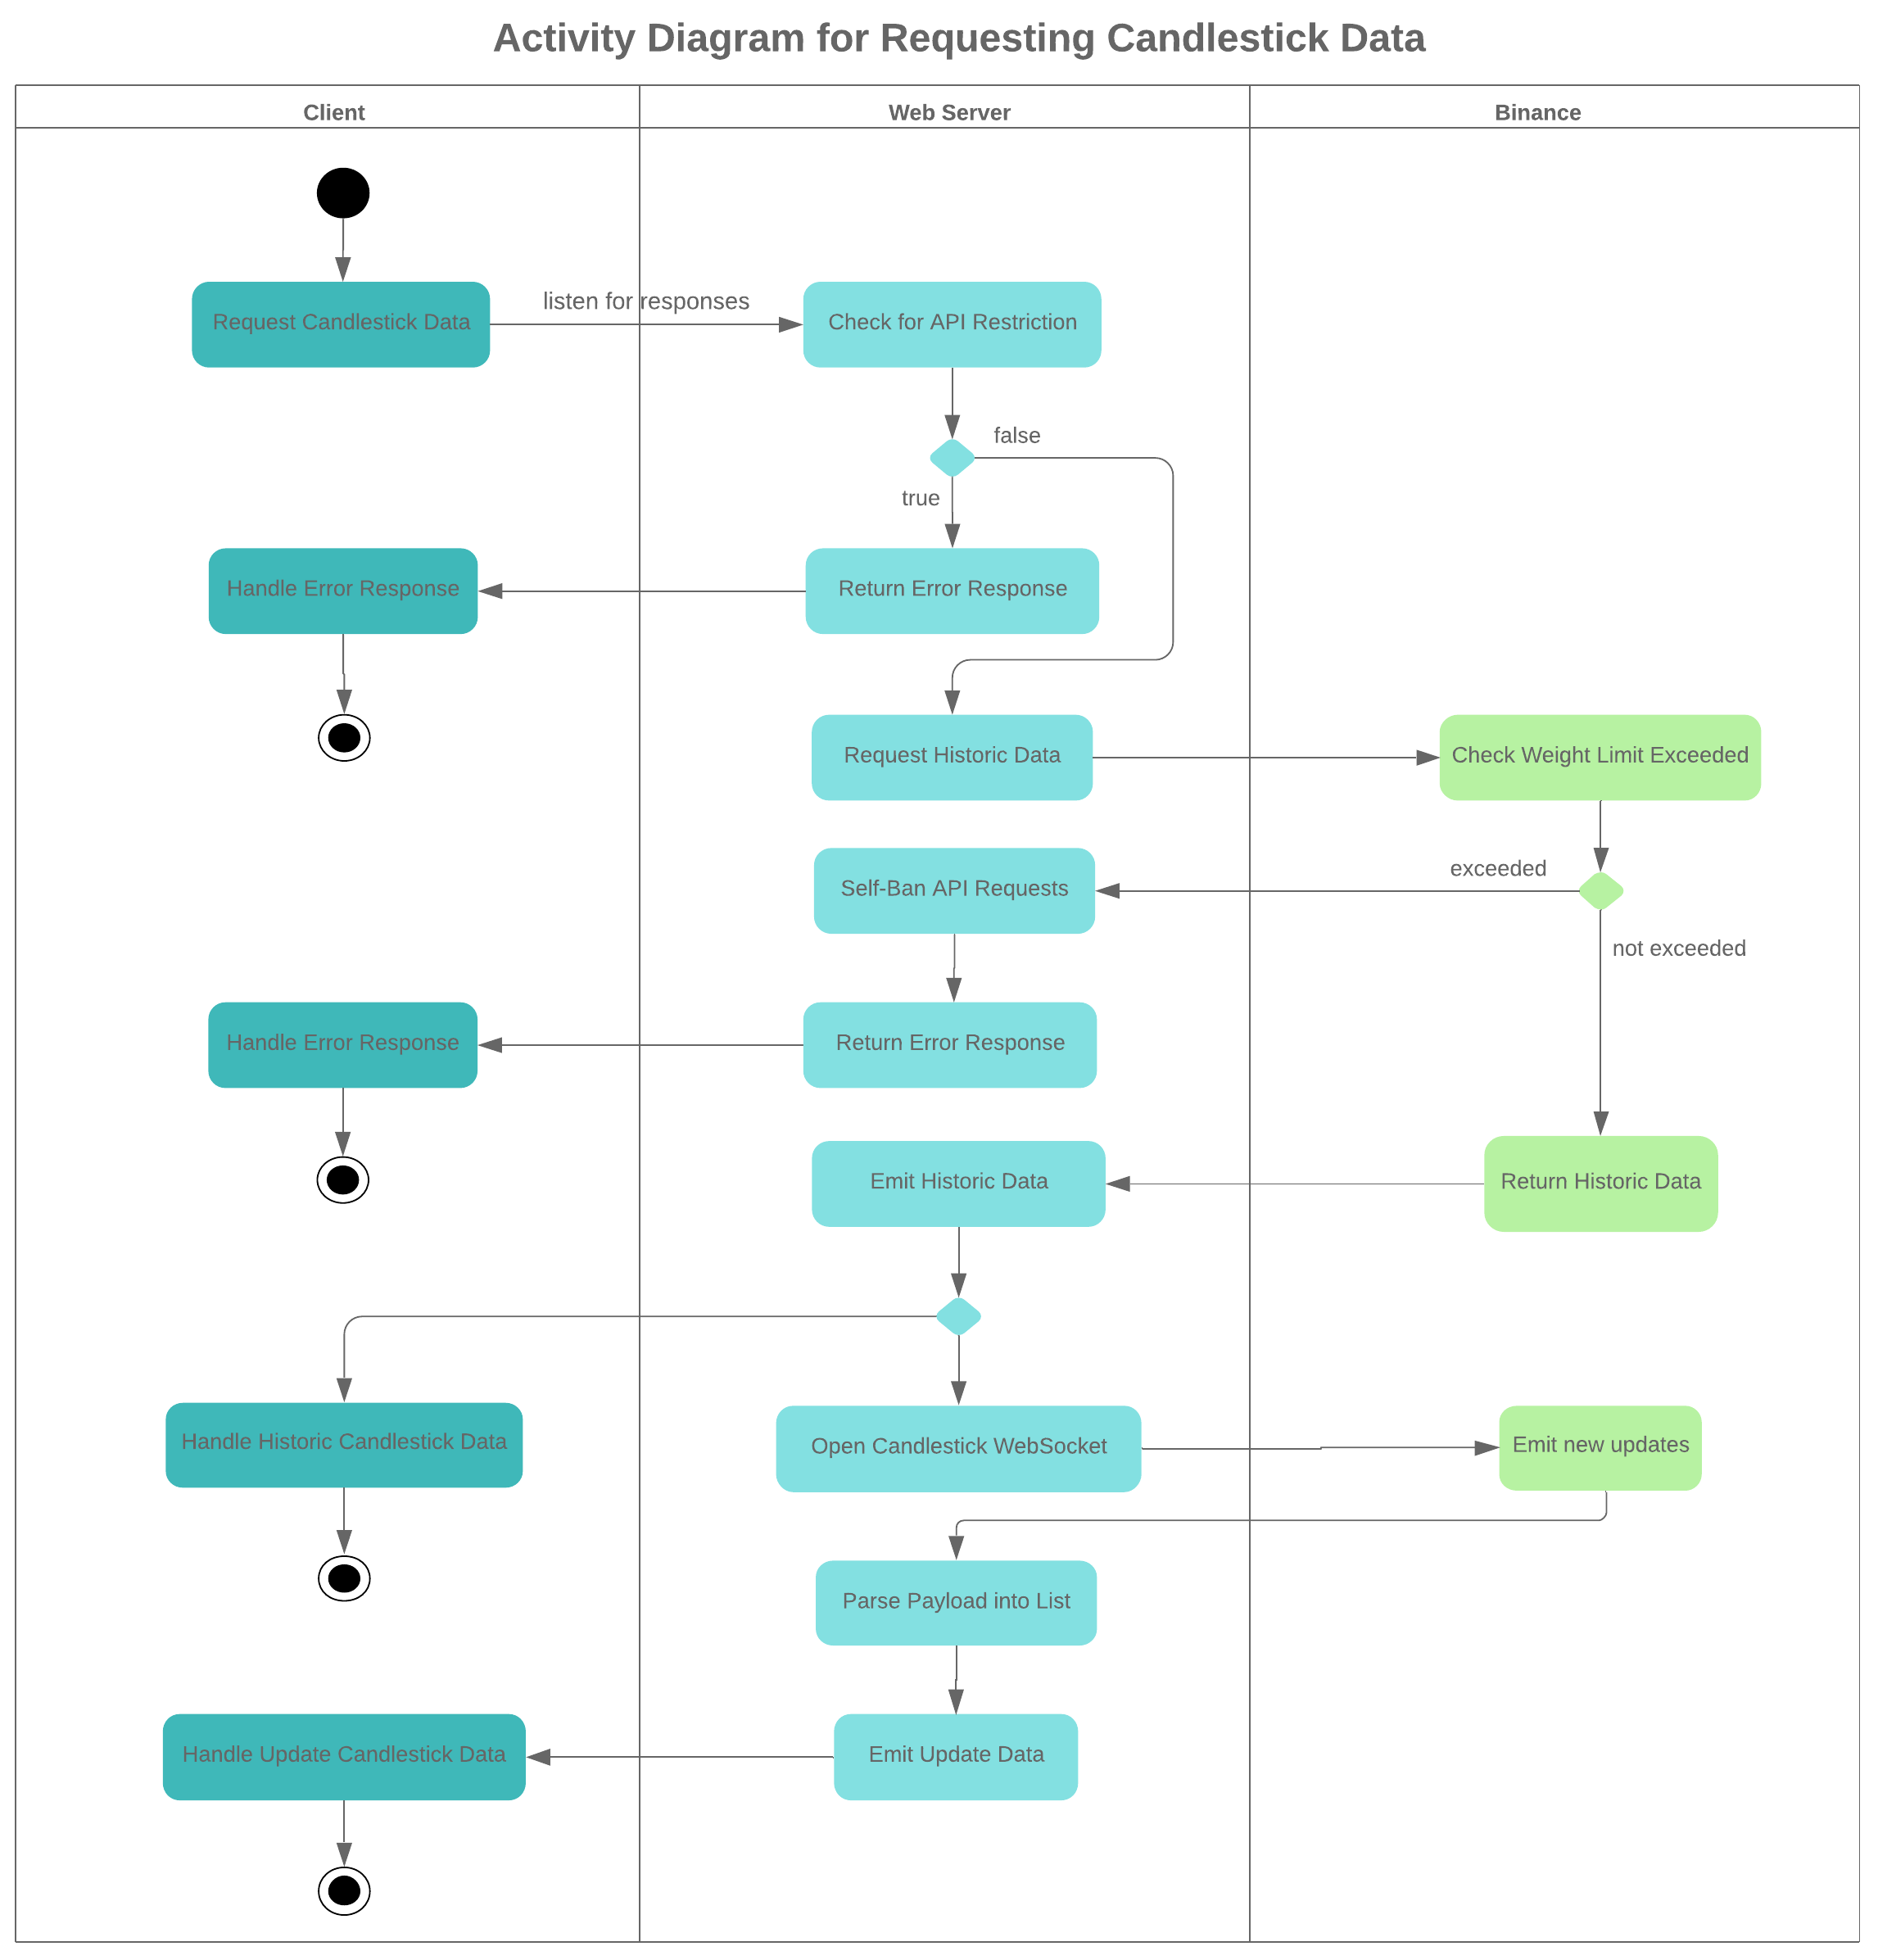
\includegraphics[width=\textwidth]{content/graphics/diagrams/AD_KLINE.png}
	\caption{Activity diagram of candlestick data: 
	\textit{(a)} The web server emits candlestick data to WebSocket client}
    
	\label{fig:implementation:actor_dataflow}
\end{figure}

Binance provide documentation of what data to expect from their endpoints regarding both the REST API and WebSocket for candlestick data. Interestingly, the data is represented differently at either endpoint with the REST endpoint returning an array of arrays (CODE SNIPPET REFERENCE) and the WebSocket endpoint returning a dictionary object (CODE SNIPPET REFERENCE). % TODO expand and state why this is an issue
For simplicity, the implemented web sever retrieves the data from both Binance endpoints and forwards this through a single WebSocket connection the user has made to the web server. This is done by the web server performing the fetch request to Binance and sending that to the user through it's own WebSocket connection. Then afterwards, starting its own WebSocket connection to Binance, mapping the dictionary to the fetch request format (SOME DATA REFERENCE) and forwarding the latest interval update to the user.

The use of streaming Binance data through their WebSockets was overlooked during the initial research phase for this project. As such, NFR-1 now has reduced significance as their is no weighting restrictions when using their WebSockets. However, as this project - in future iterations - intends to scale to serve multiple users, who on requesting candlestick data require an initial historic data request, an API restriction is used to prevent the web server's IP address from being banned. The API restriction works as the web server performs a \textit{self-ban} for the remainder of the warning interval when receiving a 429 status code from Binance. This status code signifies too many requests have been sent to Binance within the interval.

When the 429 status code triggers, the status code handler calculates when the next fetch request is allowed to be made. This is done by taking the millisecond time stamp the trigger occurred at, calculating where the start of this interval occurred at and then adding on the next minute. This can be seen at code snippet (REFERENCE CODE SNIPPET HERE). The calculated time would be added to a SQLite database stored on the web server so the restriction time could be accessible globally. At every API fetch to Binance a check of the current millisecond time being greater than the saved time in the database would occur. This process satisfies NFR-1 and is evaluated in section \ref{sec:evaluation}.

Both order book and basic overview data of all coin pairs were also used in this project. As per the initial aims of this project the order book data endpoint was going to be utilised to find suitable entry into the market, however, due to time constraints these data endpoints are now used as additions to the UX on the front end UI. These endpoints were implemented differently from the candlestick chart data endpoints by having their own dedicated URL for REST requests and their own WebSocket endpoints. This is discussed in section (TODO UPDATE REF) \ref{sec:implementation:frontend}. As both endpoints retrieve data from Binance, the API restriction handler and check are utilised.
% ADD TESTING OF ALL 3 ENDPOINTS TO PROVE API RESTRICTION

\subsection{Bot Communication \& Management}
\label{sec:implementation:info_comm:bot_comm_management}

\noindent There is two REST endpoints implemented for controlling and configuring a bot. The first endpoint is used to start a bot by passing parameters such as the coin pair, the strategy ID being used, and the parameters for that strategy. This endpoint is wrapped in a WebSocket connection as to allow the bot to stream signals to the front end after initalisation. This WebSocket is required to constantly push the latest signals to the user as they happen. A second REST endpoint is used to stop an existing bot by sending its unique hash ID.

A hash ID is the response returned from the web server when successfully starting a bot. This provides a way to uniquely identify any bot in a machine readable way. Storing a bot to be communicated with on demand was a challenge because a bot only exists in the server's memory. There was no straightforward method to storing a reference to a bot in a database that can be used to control it at a later time. Therefore, a solution to this issue was to create an \textit{existence} model that would keep the memory references to a bot's \textit{manager} model that can be retrieved using hash IDs. While this may have issues when dealing with large quantities of users, this approach is satisfactory for the scope of this project. 
% TODO maybe reword 'create a model that would store the existence of the bot in memory
% TODO Define the existence and manager model more clearly

Stopping a bot requires sending the hash ID that is generated on its initialisation as a parameter to the appropriate endpoint. This endpoint queries the \textit{existence} model by performing a look up of the hash ID. A variety of checks are performed to return the correct status code, such as if it doesn't exist.  This would illicit an appropriate response so that the UI can handle this correctly. If the bot does exist, then the bot is stopped and a further check is performed to see if it is stopped successfully. These checks are crucial to ensuring clarity about the systems current status like confirming the existence of a bot. This approach is common throughout the system and allows multiple variations of responses to be returned. The UI can then handle this appropriately to keep the user updated about the outcome of requests.
%TODO create diagram like the handshake protocol to show communication to the web server

The bot \textit{manager} model is the hub that a user interacts with through starting and stopping the bot. This model manages one bot at a time and ensures the bot process (SOME REF HERE) and dependencies are initialised correctly, there is a valid user session ID to forward the output too and the bot is fully shutdown on a stop request. Designing this model allows for multiple bots to operate concurrently, while also allowing more than one strategy to operate simultaneously.


\section{Bot Process}
\label{sec:implementation:bot}

\noindent As mentioned above, the bot process is built on \textit{actor} models for a non-blocking data flow. The initial design of this system was to have this process operate sequentially. However, during development the system would block until a long tasks would complete. This raised issues, such as the gathering of Binance data missing updates as the intensive process of generating signals was being executed. This meant crucial data could be potentially missed which would lower the effectiveness of the bot.

% socketio client, listens to existing namespace, gets intial data then receives updates thereafter
The first stage of the process was to gather the exchange data to operate the bot. Initialising a WebSocket client that would connect and listen to the web server's stream of candlestick data was the simplest solution. This is because the client listens to the already implemented name-space that pushes the data to the front end UI , which is discussed in section \ref{sec:implementation:info_comm:binance_exchange_data} (Pg. \pageref{sec:implementation:info_comm:binance_exchange_data}). This ensured consistency between the data present on the front end UI and what the bot was processing, as well as reducing code duplication and testing. The WebSocket client library handles incoming data concurrently so the actor model was not required. The data gatherer actor simply listened for new incoming data, and forwarded it to the processing actor.

The actor model used for this process is based on an \textit{inbox} system. This is a queue that actors constantly check for new \textit{messages}. When a message is received it is popped from the queue and handled accordingly. This allows for other parts of the program to execute while the actor is waiting on messages. This couples the different processes of the system by the data flow being pushed to each actor in a non-blocking way as seen in figure \ref{fig:implementation:actor_dataflow} (Pg. \pageref{fig:implementation:actor_dataflow}). 

\begin{figure}[htb]
    \centering
	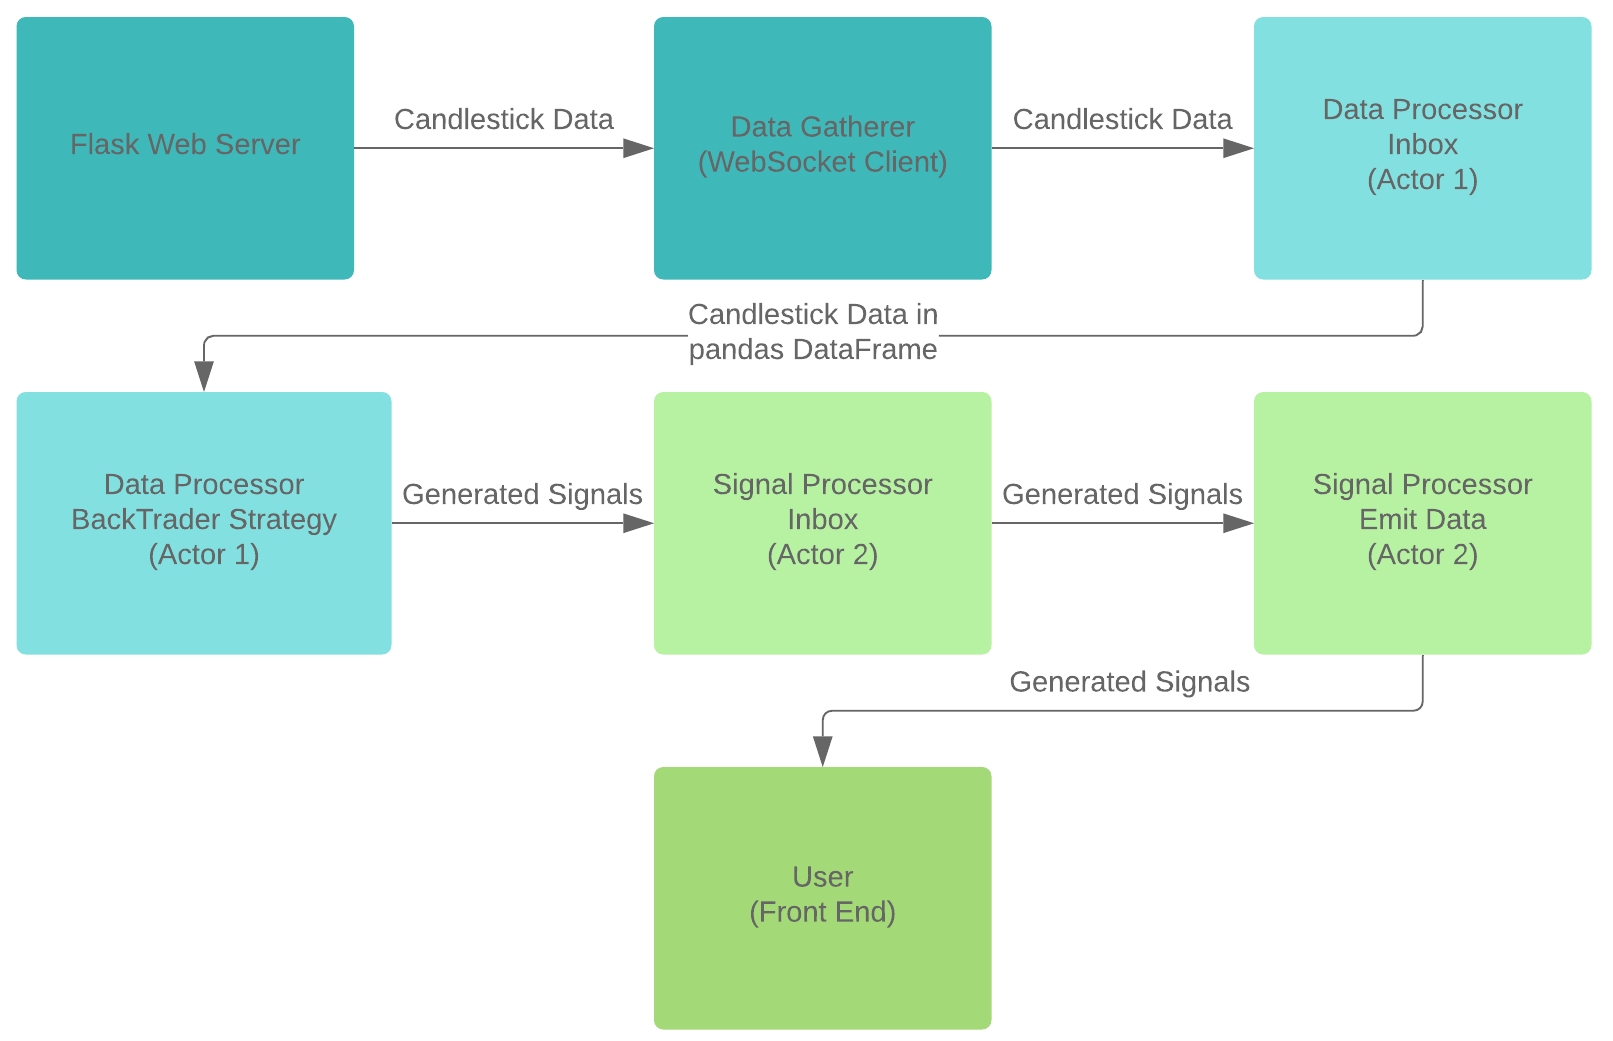
\includegraphics[width=0.9\textwidth]{content/graphics/diagrams/actor_dataflow.png}
	\caption{Data flow of the bot process: 
	\textit{(a)} The web server emits candlestick data to WebSocket client
	\textit{(b)} WebSocket client forwards data to actor 1's inbox
    \textit{(c)} Actor 1 pops data from inbox and parses data into pandas data structure
    \textit{(d)} Actor 1 executes chosen strategy using BackTrader and pushes signals to actor 2
    \textit{(e)} Actor 2 pops data from inbox passes to handler
    \textit{(f)} Actor 2 emits data to specific client}
    
	\label{fig:implementation:actor_dataflow}
\end{figure}

% data process, strategies, keeps data in memory, only updates
%maybe discuss how backtrader limitations of supporting live data from their selected brokers required work arounds?
% TODO discuss how the bot manager initalises and communicates with this process
The data processing stage is an actor and the most intensive part of the bot process. Shown in figure \ref{fig:implementation:actor_dataflow}.c, the actor receives candlestick data into its inbox. This is received as a standard python list and requires to be transformed into a pandas DataFrame. The DataFrame data structure is required as it can index and order itself by time stamp. This is extremely beneficial for manipulating time series data and why it is useful for financial software. This initial DataFrame is stored in the actor and all the following data appends or updates the latest interval data. 

The Back Trader library is utilised in the following steps of the data processor as shown in figure \ref{fig:implementation:actor_dataflow}.d. The strategy and its parameters that were given to the manager model are executed on the pandas DataFrame. Back Trader applies the strategy on the data and generates signals when signal conditions are met. The signals are then returned as the result of executing the strategy.

% TODO update listed indicators based on strategies made
The strategies used for this project are designed using the technical indicators discussed in section \ref{sec:related:tradingStrategies}, such as the \textbf{SMA}, \textbf{RSI}, \textbf{MACD} and \textbf{Bollinger Bands}. The indicators are provided by the Back Trader library and can be easily imported into the strategy (CODE SNIPPET HERE). Trade signals occur when conditions of all the indicators in the strategy are met. In the case of the \textbf{SMA Crossover \& RSI} strategy, by default a buy signal occurs when the RSI is below 30 and the smaller 15 interval SMA crosses above the longer 30 interval SMA (MAYBE CODE SNIPPET). Defining a strategy is relatively straightforward with Back Trader as manipulation and conditional checks can be used like other natural programming constructs.

% TODO discuss all the implemented strategies

Handling the variation on the number of parameter options between signals required a standard between the data processor, the web server's bot communicator and the front end UI. This is to ensure that the inputs of a parameter entered on the UI correspond with the correct parameter in the strategy. To tackle this, dictionary objects were used to look up the parameter's value by a key. For the scope of this project, the keys were string versions of integers from 1 to N (N being the number of parameters for the signal). Using a dictionary allows the keys to change and update appropriately when the complexities of strategies are increased, improving on maintainability in future iterations of the project.

% signal handling process, emit to correct user
% TODO maybe showcase websocket SID is valid and how this actor handles that
The last actor used in the bot process is the signal processor seen in figure \ref{fig:implementation:actor_dataflow}.e and \ref{fig:implementation:actor_dataflow}.f. The bot manager initialises this actor with the user's WebSocket session ID so the actor can emit signals to the correct users. This actor is designed to forward data to the correct user and validate that there is a user to receive the signals. It tackles this problem by confirming that there is an SID and there is an active connection to the user. 

Overall, the actor model is beneficial towards the development of this project by providing a non-blocking flow of data between the main components of the bot shown by figure \ref{fig:implementation:actor_dataflow}. This model circumvents the intensive signal generation process that the data processor requires, while being able to continually listen for new data being received from the web server. Strategies can be easily slotted into the data processor by modular design of the data processor. 



\section{Front End Process}
\label{sec:implementation:frontend}

% TODO add react and redux to lit review
\noindent Implementation of the front end can be categorised into two main sections, data visualisation of Binance's market data, and user controls and notifications of the platform. Both sections utilise two main technologies, React and Redux. As discussed in section \ref{sec:design:frontend} (Pg. \pageref{sec:design:frontend}), Redux is an \textbf{application state manager} and React is a \textbf{UI library}. Both technologies integrate well together, with React creating self-contained components and Redux tying them together with a central \textit{store}.

% Quick redux example, react example
Redux was necessary to allow actions of controllers update the rest of the UI. For example, selecting a different coin pair such as ETH/USDT would trigger an action to update the store's state to what the current coin pair is selected. This would then cause the candlestick chart, order book, quick information panel and bot controller options to update. 

% Data Visualisation of Market Data Section
\subsection{Data Visualisation of Market Data}
\label{sec:implementation:frontend:data_vis}
%% Candlestick/Volume
\noindent The main area of the front end UI is the candlestick chart. This chart can visualise current and historic price information of a coin pair. It displays information on the open and close and highest and lowest prices within an interval. The chart itself is a library that is heavily customisable and requires data to be passed into it. The logic for data retrieval is implemented in a container that then renders the chart. When the container is mounted, a WebSocket is opened to the web server to request data. This request takes the current coin pair saved in the Redux state - BTC/USDT by default - and requests the streaming of data. The container then \textit{listens} for the response which is then parsed and pushed into the chart component which populates the chart intervals.

% Maybe code snippet of mapping function and data retrieved?
Parsing the retrieved data uses a mapping function to transform a list into a JavaScript object. The millisecond time stamp is converted to a UTC string date\footnote{e.g. Fri, 02 Feb 1996 03:04:05 GMT} and assigned to a key-value pair in a JavaScript object, along with the open, close, highest, lowest and volume data indexes in the list. Performance may suffer on weak systems when large amounts of data is required to be parsed to this format. While performance issues did not occur on development systems, this may be worth further investigating in future iterations. 

One solution to performance issues could include prepossessing the required format on the server before the user retrieves the data, however this would then cause inconsistencies between data formats. A data parameter could be used to toggle the prepossessed format in future iterations. It is worth noting that the intense mapping operation only occurs on the initial received data due to the web server forwarding the historical data. The data received thereafter is used for appending or updating the latest interval. This is discussed in depth in section \ref{sec:implementation:info_comm:binance_exchange_data} (Pg. \pageref{sec:implementation:info_comm:binance_exchange_data}).

Unfortunately, due to time constraints, implementation of technical indicators corresponding to the indicators a strategy would use was missed within the time line of this project. This could be implemented in future iterations, however, the \textbf{SMA} and \textbf{Bollinger Band} indicators are displayed on the chart as placeholders. Further developing the UI to align with the bot's strategy would offer the user more information of how the bot derived signals from it's indicators.

%% Orderbook
Within the bot's signal generation process, the order book is not used to perform trade executions as this feature is outside the scope of this project. However, the UI implementation brings information about the market's depth to the user and can display how liquid or illiquid a market is. Developing the order book had challenges to ensure the data displayed is accurate with no missing pieces.

Ensuring this firstly required streaming data from the WebSocket into a buffer that holds data representing \textit{updates} to the current order book. After receiving the first payload from the WebSocket, a fetch request for the order book's historical data is sent. After receiving the response data, the streamed data residing in the buffer with a time stamp older (smaller) than the historical data's time stamp is discarded. The historic data is then placed in the buy or sell order book table and the rest of the order book buffer is emptied to update the tables. All new streamed data is then able to update these tables, and ensures the buy and sell order books are accurate and up-to-date.

%% Quick Info Panel
For a quick overview of the market conditions, a data panel is provided at the top of the UI providing information such as the current coin price, what coin pair is currently being viewed, the volume traded within the last 24 hours and other useful information. This panel is managed entirely by the Redux state manager and is the main point of reference to feedback meta information the user is currently looking at. All the data is collected and updated from different components of the UI, displaying the web app's overall state.

% User Controls and Notifications
\subsection{User Controls and Notifications}
\label{sec:implementation:frontend:controls_notifications}
%% Bot Controls
% TODO pretty weak intro, fix it
\noindent The bot control panel has two main points of functionality, toggling the bot on or off and configuring the bot through strategy selection. By implementing the strategies and their configurations directly into the front end has increased difficulty for future maintainability and addition of strategies. As strategies are written directly into the Redux state, updating or adding a strategy requires that they are also updated on the web server. This means that updates to the strategies require change in two different parts of the application. In future work, implementing an endpoint that the front end can request all offered strategies and their configurations would reduce the time required to add or update strategies.

The strategy selection and configuration panel provides a drop down box of strategies that are currently offered. Selecting a strategy displays parameters specific to that strategy and which the user may customise. These configuration options are sent to the server when starting the bot. After requesting a bot to start, the bot's hash ID is returned as the initial response. This hash ID is stored on the front end to allow the user to stop the bot at a later point. Their is limitations towards the current implementation as it can only store one hash ID and store this ID during the current browser session. This provides limitations towards future goals of controlling multiple bots simultaneously.

One solution would be to create a login and account management system where a bots hash IDs can be attached to an account and stored in a database. This would create persistence of controlling the bot between web browser sessions by being able to retrieve the hash IDs on login and allowing multiple bot IDs to be controlled. 

%% Push Message Panel
Keeping the user up-to-date with the current status and operations of the bot led to implementing two types of notifications. The first being a push message panel that creates a log of vital system messages that can communicate the current status and intent of a bot. Messages in this panel can be generated by both the front end and the web server. The second being \textit{snackbar} notifications that provide system confirmations for convenience, providing feedback to the user that their actions have been processed. The snackbar implementation is provided by material-ui and offers colour coded message types. This offers different information to the user through success, warning, error and information messages.



%% Coin pair selection

%% Page Selection???






